\subsection{Configuration Parameters}

\begin{frame}{Command-Line Options}
	\leftorright{
		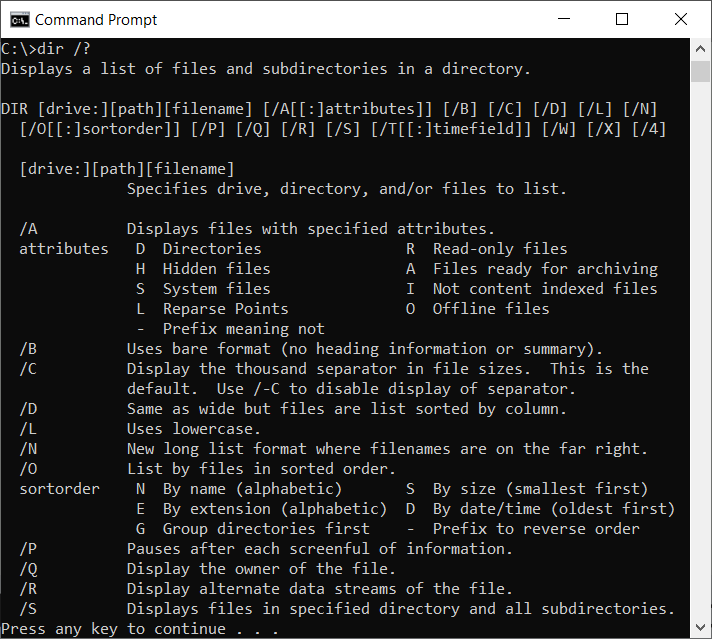
\includegraphics[width=\linewidth]{runtime-parameters-win10-cmd-dir}
	}{
		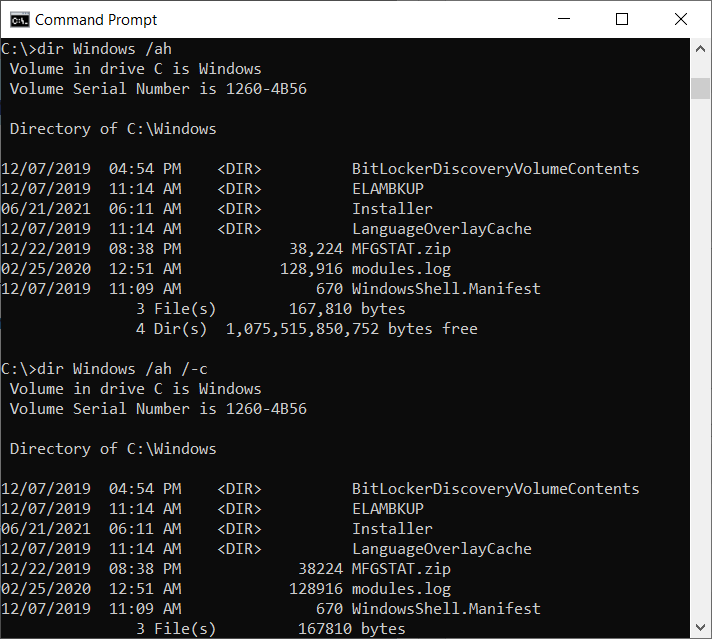
\includegraphics[width=\linewidth]{runtime-parameters-win10-cmd-dir2}
	}
\end{frame}

\begin{frame}{Configuration Files}
	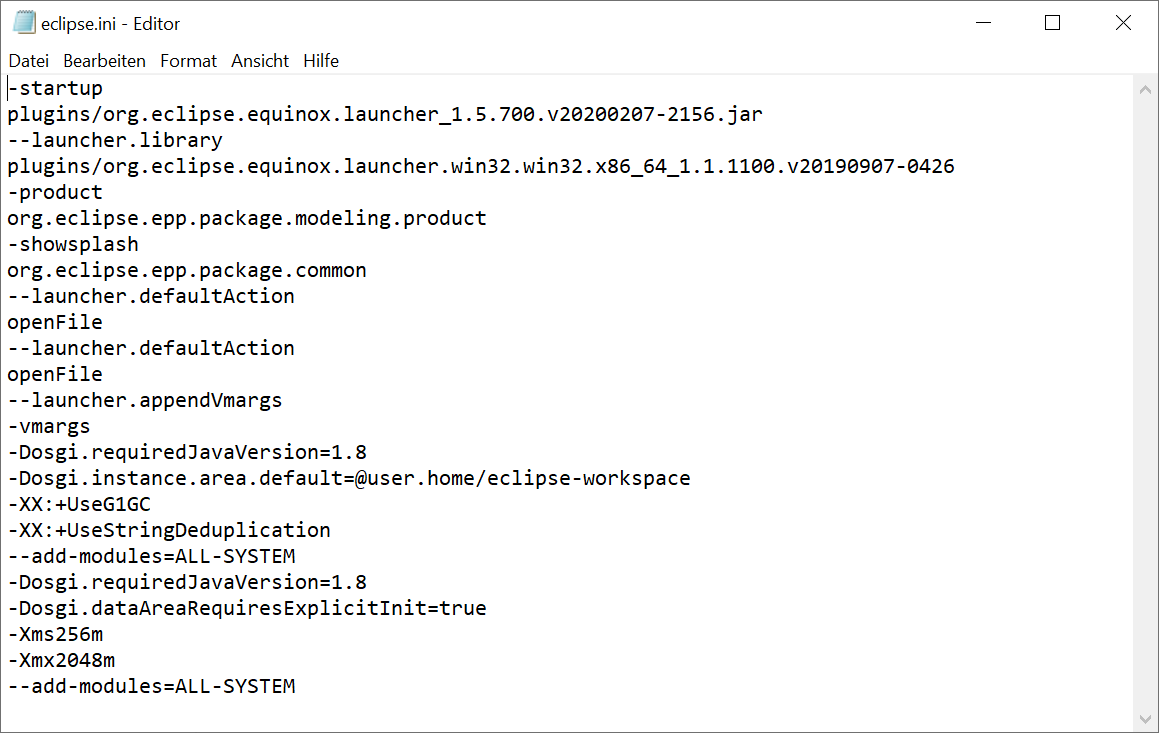
\includegraphics[width=0.75\linewidth]{configfile-eclipse-ini}
\end{frame}

\begin{frame}{Preference Dialogs}
	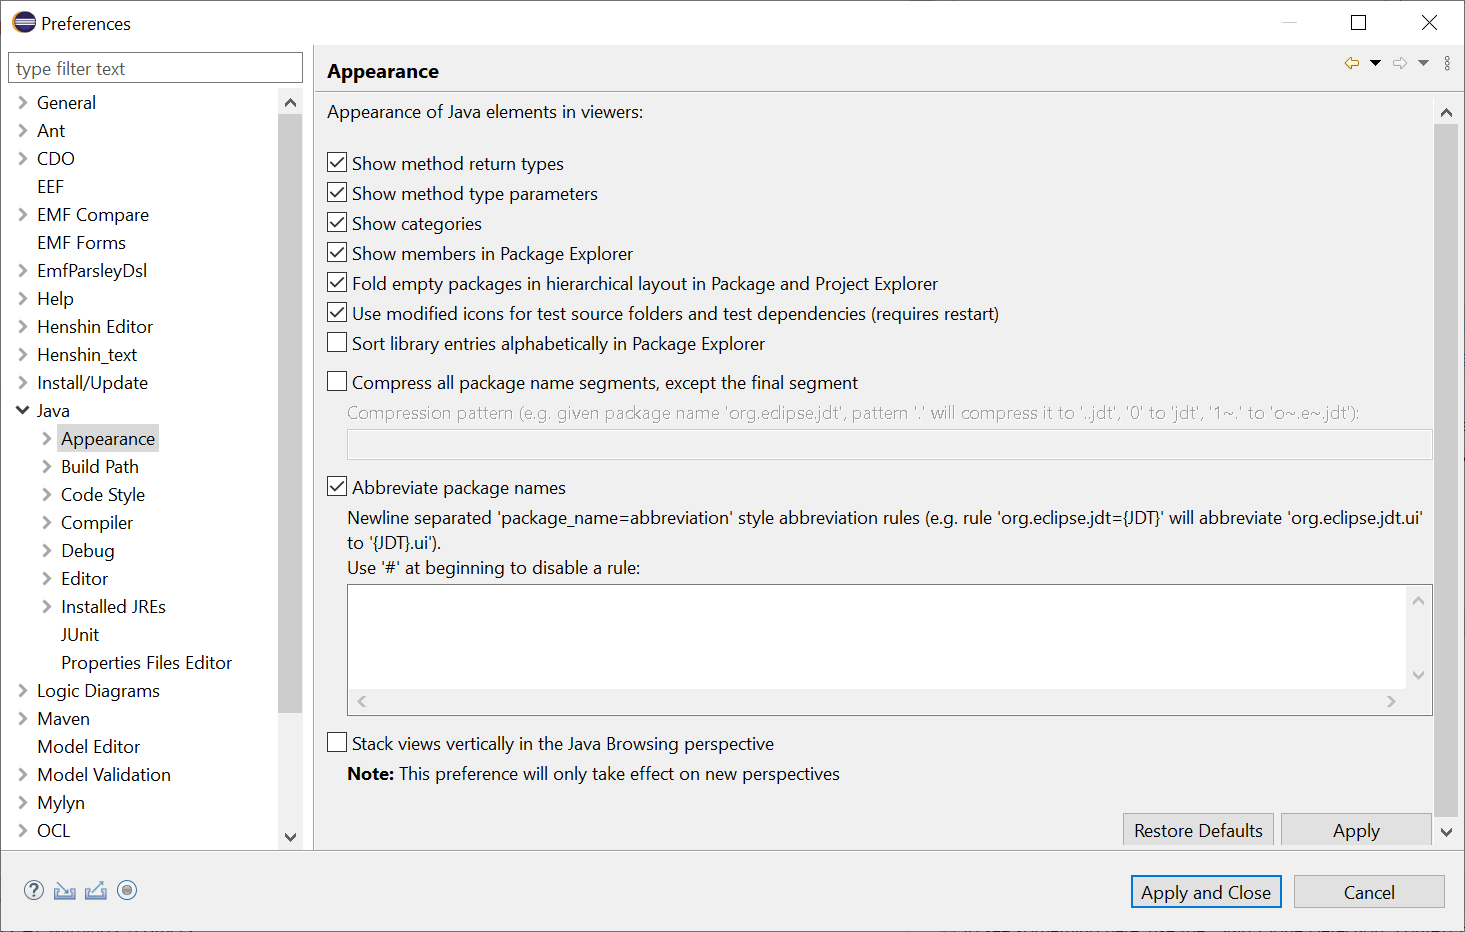
\includegraphics[width=0.75\linewidth]{preferences-eclipse}
\end{frame}

\begin{frame}{Common Principle: Runtime Variability}
	\leftorright{
		\myexampletight{Command-Line Options}{
			\begin{center}
				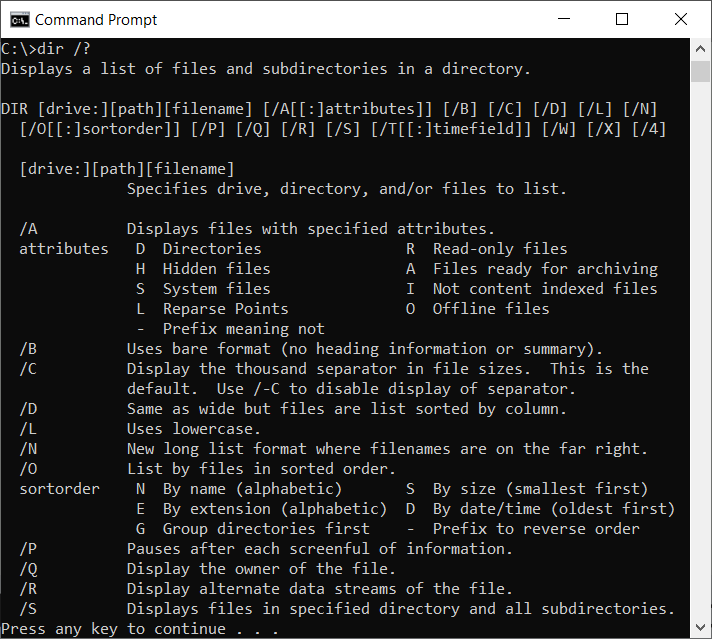
\includegraphics[width=0.7\linewidth,height=0.125\textheight]{runtime-parameters-win10-cmd-dir}
			\end{center}
		}
		\myexampletight{Configuration Files}{
			\begin{center}
				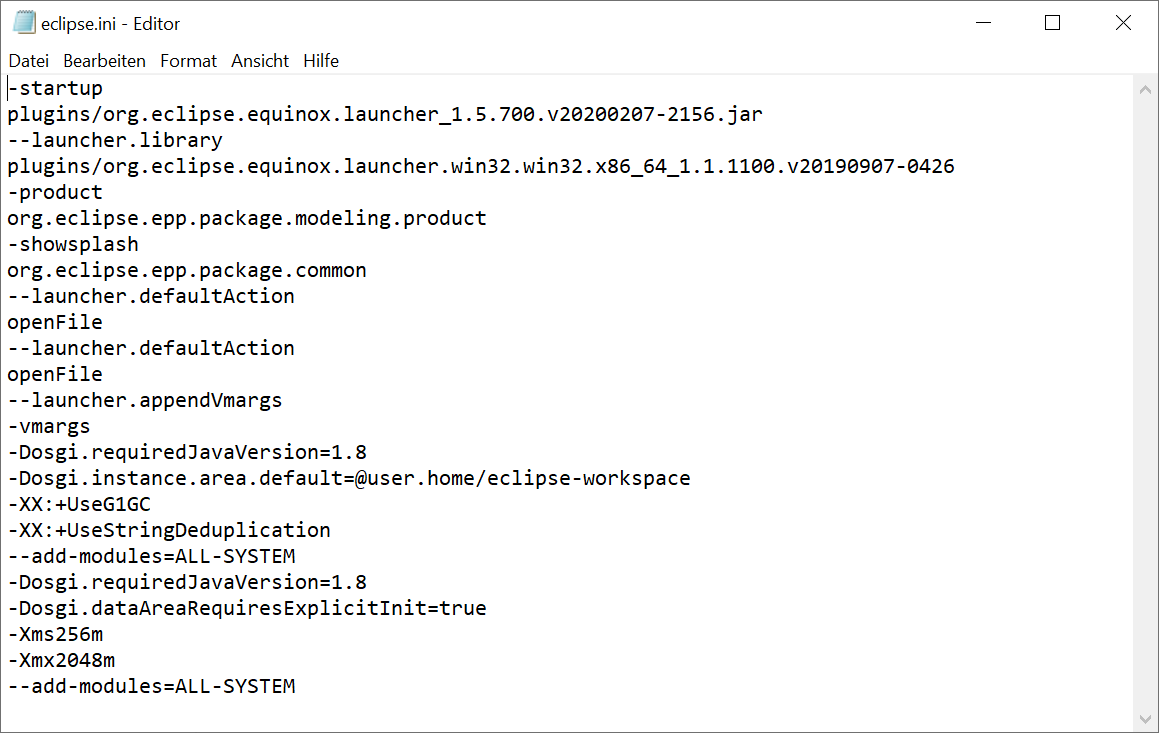
\includegraphics[width=0.7\linewidth,height=0.125\textheight]{configfile-eclipse-ini}
			\end{center}
		}
		\myexampletight{Preference Dialogs}{
			\begin{center}
				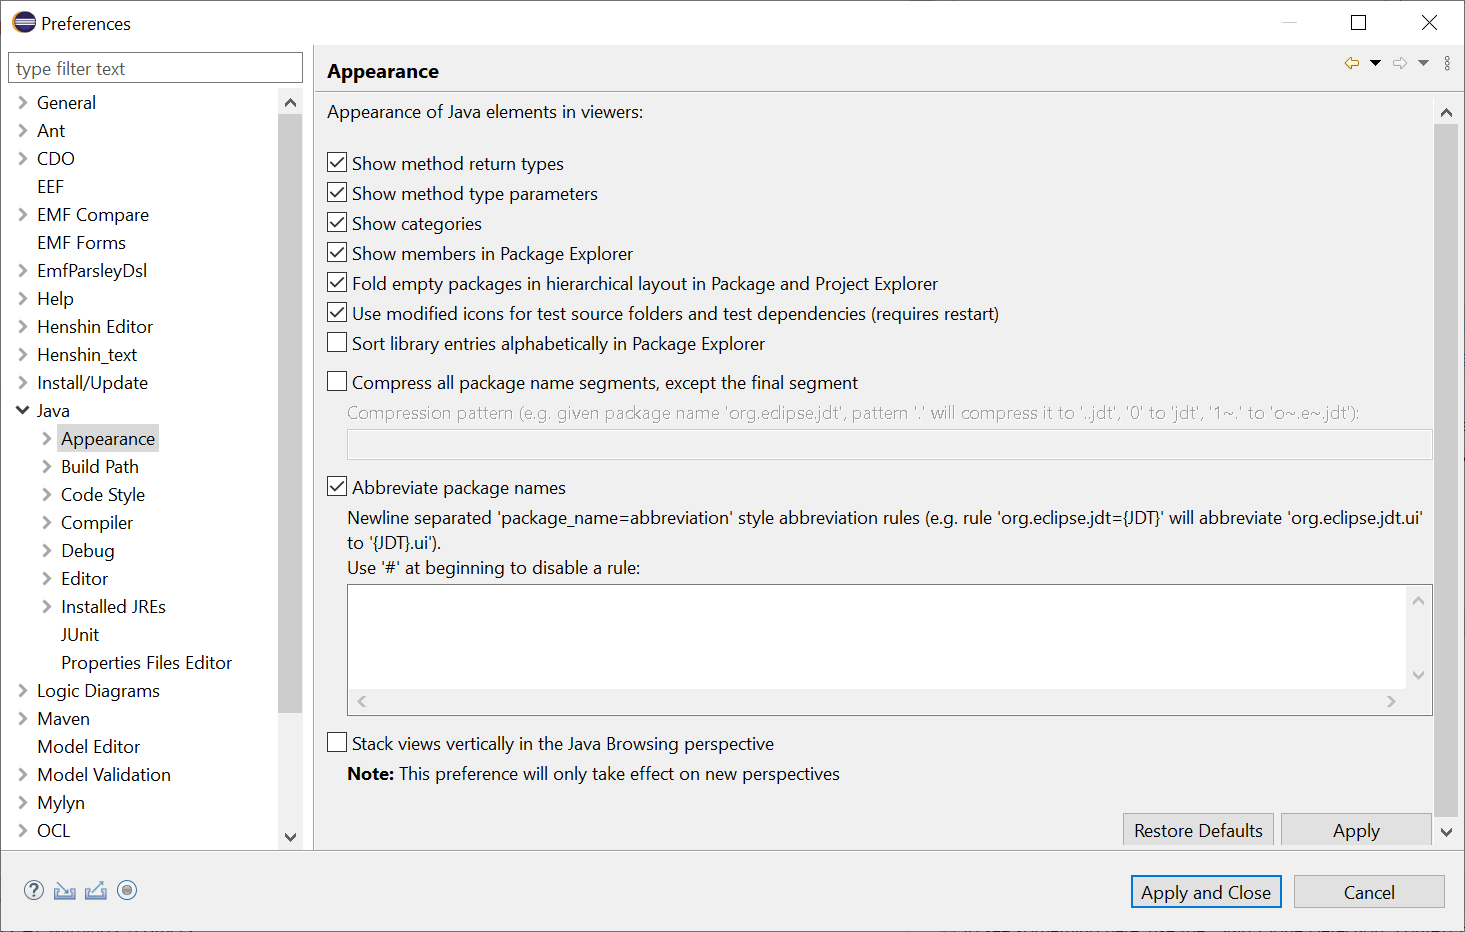
\includegraphics[width=0.7\linewidth,height=0.125\textheight]{preferences-eclipse}
			\end{center}
		}
	}{
		\mynote{Configuration Parameters}{
			\begin{itemize}
				\item Behavior of a program is determined by configuration parameters being interpreted at runtime.
				\item Configuration may happen non-interactively (at startup) or interactively (through dialogs).
			\end{itemize}
		}
	}
\end{frame}

\subsection{Example: A Graph Library}

\begin{frame}{\myframetitle}
	A simple library providing \ldots \\
	\vspace{5mm}
	\leftorright{
		\myexample{\ldots graph data structures}{
			\begin{itemize}
				\item Directed/undirected edges
				\item Weighted/unweighted edges 
				\item Colored/uncolored nodes
				\item etc.
			\end{itemize}
		}		
	}{
		\myexample{\ldots and algorithms}{
			\begin{itemize}
				\item Vertex numbering
				\item Vertex coloring 
				\item Shortest path
				\item Minimum spanning tree 
				\item etc.
			\end{itemize}
		}
	}
\end{frame}

\subsection{Features as Configuration Parameters}
\begin{frame}{Features of a Graph as Configuration Parameters}
	\leftorright{
		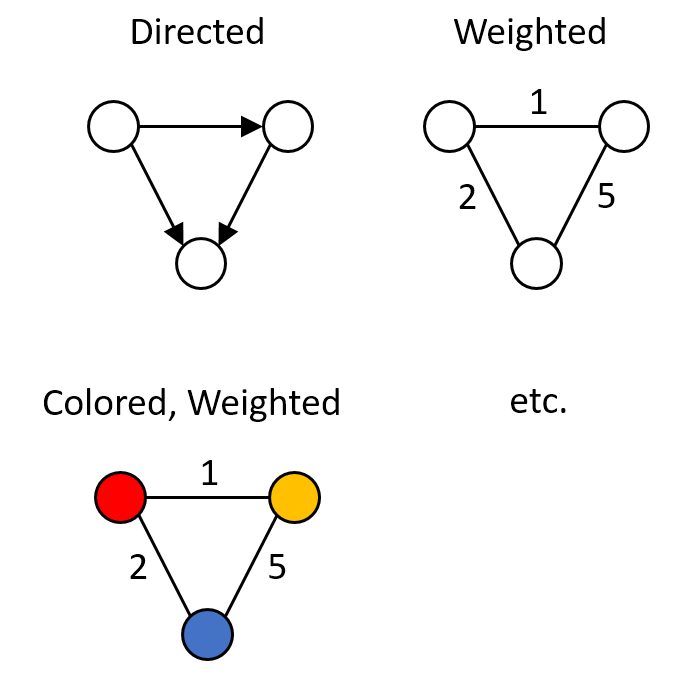
\includegraphics[width=0.9\linewidth]{graph-features}
	}{
		\mynote{}{
			\begin{itemize}
				\item Typically, configuration parameters are flags.
				\item Their boolean value determines which features are activated and which ones are deactivated.
			\end{itemize}
		}
	}
\end{frame}





\subsection{Validity of Parameter Settings}
\begin{frame}{\myframetitle}
	\begin{columns}
		\column{.6\textwidth}
			\begin{tabular}{llll}
			\toprule
			{\bf Algorithm} 							& {\bf Graph type} 	& {\bf Weights} & {\bf Coloring}  \\ \midrule
			{\em Vertex numbering}			  & *          				& *        			& *         			\\
			{\em Vertex coloring}       	& undirected 				& *        			& colored   			\\
			{\em Shortest path}        		& directed   				& weighted 			& *         			\\
			{\em Minimum spanning tree} 	& undirected 				& weighted 			& *         			\\
			\ldots         					& \ldots 			 			& \ldots 		  	& \ldots 					\\ \bottomrule
			\end{tabular}
			\vspace{5mm}	
			\mynote{Dependencies between features must be checked}{
				\begin{itemize}
					\item When the parameters are configured at startup, or
					\item whenever parameters are changed at runtime.
				\end{itemize}
			}
		\column{.35\textwidth}
			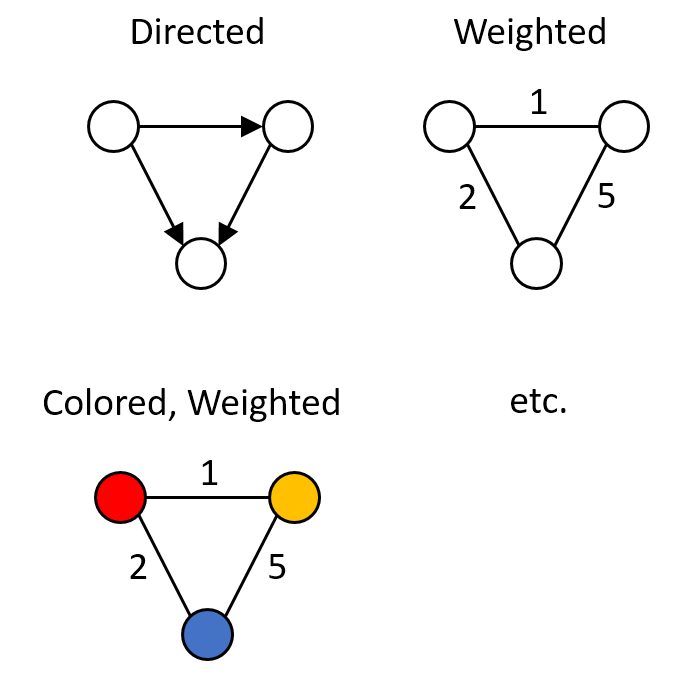
\includegraphics[width=\linewidth]{graph-features}
	\end{columns}
\end{frame}

